%
% Finite Elemente
%
\section{Finite Elemente
\label{buch:pdenumerik:section:fem}}
Die Methode der finiten Differenzen verwendet die Funktionswerte
in den Gitterpunkten, um die Ableitungen durch Differenzenquotienten
zu approximieren.
Dies entspricht einer linearen Approximation der Funktion zwischen
den Gitterpunkten.
Die Methode der finiten Elemente versucht, die Werte in den
Gitterpunkten dazu zu verwenden, eine Approximation der Lösungsfunktion
zu konstruieren, die auch zwischen den Gitterpunkten eine gut ist.
Sie kann zusätzlich auch Ableitungswerte in den Gitterpunkten als
Unbekannte verwenden.
Die Konstruktion der linearen Gleichungen wird etwas komplizierter,
sie verwendet Integrale über die Intervalle oder Gebiete zwischen
den Gitterpunkten.
Dies ermöglicht, eine sehr gute Approximation mit einer vergleichsweise
kleinen Zahl von Gitterpunkten zu konstruieren.

%
% Schwache Form der Differentialgleichung
%
\subsection{Schwache Form der Differentialgleichung}
Zur Illustration der Idee der Methode der finiten Elemente verwenden wir
als Beispiel die eindimensionale Differentialgleichung
\begin{equation}
u''(x) = f(x)
\label{buch:pdenumerik:fem:eqn:u2}
\end{equation}
auf dem Intervall $[a,b]$.
Dies ist der eindimensionale Fall der Laplace-Gleichung $\Delta u = f$.

%
% Skalarprodukt
%
\subsubsection{Skalarprodukt}
Die Gleichung \eqref{buch:pdenumerik:fem:eqn:u2} ist gleichbedeutend
mit $u''(x)-f(x)=0$.
Es geht also darum, Bedingungen aufzustellen, die garantieren können,
dass $u''(x()-f(x)=0$ ist.
Eine Analogie zur Vektorgeometrie kann helfen zu verstehen, wie dies 
gelingen kann.
Ein Vektor $\vec{v}\in\mathbb{R}^n$ verschwindet, wenn jede einzelne
Komponente $=0$ ist.
Das ist die lokale Betrachtungsweise der Methode der finiten Differenzen.
Man kann aber auch eine beliebige Basis $\vec{b}_1,\dots,\vec{b}_n$ nehmen
und als Bedingung stellen, dass 
\[
\vec{v}\cdot\vec{b}_k = 0
\]
ist für $k=1,\dots,n$.

Auf die Gleichung \eqref{buch:pdenumerik:fem:eqn:u2} übertragen
bedeutet dies, dass wir zunächst ein Skalarprodukt für Funktionen
auf dem Intervall $[a,b]$ benötigen.
Das $L^2$-Skalarprodukt
\[
\langle f,g\rangle
=
\int_a^b f(x)g(x)\,dx
\]
bietet sich hier für an.
Dieses Skalarprodukt lässt sich auch für
ein beliebiges kompakte Gebiet $G\subset\mathbb{R}^n$ definieren.

Als nächstes wird eine Familie $g_i(x)$ von Funktionen benötigt, mit
denen man die Bedinungen $\langle u''-f,g_i\rangle=0$
formulieren kann.
Und schliesslich braucht es eine Approximationsfunktion für $u$, die zweimal
differenzierbar ist und für die man das Skalarprodukt berechnen kann.

%
% Reduktion der Ordnung mit partieller Integration
%
\subsubsection{Reduktion der Ordnung mit partieller Integration}
Die gesuchten Approximationsfunktion, aus denen eine Approximation von
$u(x)$ zusammengebaut werden kann, scheinen zweimal stetig differenzierbar
sein zu müssen, damit $\langle u''-f,g_i\rangle$ überhaupt definiert ist.
Wenn die Funktionen $g_i$ stetig differenzierbar sind, dann kann man
mit partieller Integration das Skalarprodukt
\begin{align*}
\langle u'',g_i \rangle
&=
\int_a^b u''(x)g_i(x)\,dx
\\
&=
\Bigl[ u'(x) g_i(x) \Bigr]_a^b
-
\int_a^b u'(x) g'_i(x)\,dx
\\
&=
\Bigl[ u'(x) g_i(x)\Bigr]_a^b
-
\langle u', g'_i\rangle
\end{align*}
umwandeln.
Dieser Ausdruck ist wohldefiniert selbst wenn die Funktionen $u$ und $g_i$
nur einmal stetig differenzierbar sind.

%
% Schwache Form der Gleichungen
%
\subsubsection{Schwache Form der Gleichungen}
Wir nehmen jetzt an, dass die Funktion $u(x)$ als Linearkombination
\[
u(x) 
=
\sum_{k=1}^n a_k h_k(x)
\]
der Funktionen $h_i(x)$, mit $i=1,\dots,n$ geschrieben werden kann.
Setzt man diesen Ansatz in die Bedingung $\langle u''-f,g_i\rangle=0$ ein,
findet man
\begin{align}
\langle u''-f,g_i\rangle
=
\sum_{k=1}^n
u_k
\Bigl[h'_k(x) g'_i(x)\Bigr]_a^b
-
\sum_{k=1}^n
u_k
\langle h'_k,g'_i\rangle
-
\langle f,g_i\rangle
&=
0
\notag
\\
\sum_{k=1}^n
\Bigl(
\underbrace{
\bigl[h'_k(x)g'_i(x)\bigr]_a^b
-
\langle h'_k,g'_k\rangle
}_{\displaystyle =  a_{ik}}
\Bigr)
{\color{darkred}u_k}
&=
\langle f,g_i\rangle.
\label{buch:pdenumerik:fem:eqn:gleichungen}
\end{align}
Dies ist ein lineares Gleichungssystem für die Unbekannten $u_k$
mit der Koeffizientenmatrix $a_{ik}$ und rechten Seiten
$\langle f,g_i\rangle$.
Es kann aufgestellt werden, sobald die Funktion $g_i$ und $h_k$ festgelegt
sind.

%
% Approximationsfunktionen
%
\subsection{Approximationsfunktionen}
Zur erfolgreichen Durchführung der Methode der finiten Elemente
werden zwei Familien von Funktionen $g_i$ und $h_k$ benötigt.
Damit die Lösung der Gleichungen effizient wird, sollten die 
Funktionen sehr kleinen Träger haben, so dass nur jeweils wenige
Paare von Funktion $h'_k$ und $g'_i$ nichtverschwindendes Skalarprodukt
haben.

\subsubsection{Lineare Elemente}
Damit die Resultate einfach interpretiert werden können, sollte es
einen einfachen Zusammenhang zwischen den Koeffizienten $a_k$ und
den Funktionswerten geben.
Besonders leicht wird dies, wenn die $a_k$ wieder Funktionswerte
von $u$ auf den Punkten eines Gitters wie im
Abschnitt~\ref{buch:pdenumerik:fdm:subsection:1d} sind.
%
% fig-linear.tex
%
% (c) 2025 Prof Dr Andreas Müller
%
\begin{figure}
\centering
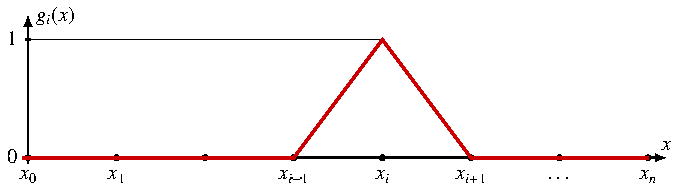
\includegraphics{chapters/090-pdenumerik/images/linear.pdf}
\caption{Die stückweise linearen Approximationsfunktionen $g_i(x)$
sind genau im Gitterpunkt $x_i$ von $0$ verschieden, wo der Wert $1$ ist,
und verschwinden in allen anderen Gitterpunkten.
\label{buch:pdenumerik:fem:fig:linear}}
\end{figure}
%
Die stückweise linearen Funktionen
\[
g_i(x_l) = \begin{cases}
1&\qquad i=l \\
0&\qquad i\ne l,
\end{cases}
\]
die auch in Abbildung~\ref{buch:pdenumerik:fem:fig:linear}
dargestellt sind.
Diese Funktionen können auch für die $h_k$ verwendet werden.

\subsubsection{Kubische Elemente}
Für die Differentialgleichung sind aber auch noch die 
Ableitungen der Funktionen nötig.
%
% fig-kubisch.tex
%
% (c) 2025 Prof Dr Andreas Müller
%
\begin{figure}
\centering
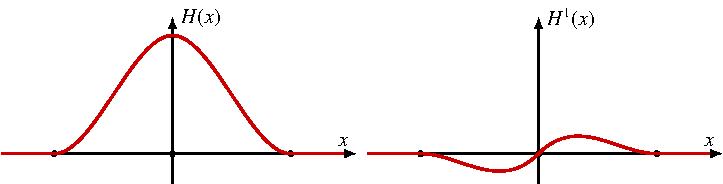
\includegraphics{chapters/090-pdenumerik/images/kubisch.pdf}
\caption{Kubische Approximationsfunktionen für die Methode der
finiten Elemente in einer Dimension.
Für ganzzahlige Argumente (schwarze Punkte auf der $x$-Achse)
hat die Funktion $H(x)$ nur bei $x=0$ den Wert $1$, alle anderen
Funktionswerte und alle Ableitungen verschwinden.
Die Funktion $H^1(x)$ ist in allen Gitterpunkten ebenso wie
ihre Ableitung $=0$ mit Ausnahme des Punktes $x=0$, wo die
Ableitung $=1$ ist.
\label{buch:pdenumerik:fem:fig:kubisch}}
\end{figure}
%
Die kubischen Funktionen 
\[
g_i(x)
=
H\biggl(\frac{x-x_i}{h}\biggr)
\qquad\text{mit} \qquad
H(x)
=
\begin{cases}
(1-2x)(1+x)^2    &\qquad -h\le x \le 0\\
(1+2x)(1-x)^2    &\qquad 0\le x \le h\\
0                &\qquad\text{sonst,}
\end{cases}
\]
die auch in Abbildung~\ref{buch:pdenumerik:fem:fig:kubisch}
dargestellt sind, sind stetig differenzierbar, haben aber
in den Gitterpunkten verschwindende Ableitungen, sie können daher
die Ableitungen der Lösungsfunktion nicht wiedergeben.

Nimmt man aber noch die Funktionen
\[
g^1_i(x)
=
hH^1(x)
\qquad\text{mit}\qquad
H^1\biggl(\frac{x-x_i}{h}\biggr)
=
\begin{cases}
x(1+x)^2         &\qquad -h\le x \le 0\\
x(1-x)^2         &\qquad 0\le x \le h\\
0                &\qquad\text{sonst}
\end{cases}
\]
hinzu, die ebenfalls in Abbildung~\ref{buch:pdenumerik:fem:fig:kubisch}
dargestellt sind, dann können auch Ableitungen wiedergegeben werden.
Die Funktionen $g_i^1$ haben nämlich im Punkte $x_i$ die Ableitung
\[
g^{1\prime}_i(x)\big|_{x=x_i}
=
H^{1\prime}(x)\big|_{x=0}
=
\bigl(
(1+x)^2+2x(1+x)
\bigr)\big|_{x=0}
=
1,
\]
während die Funktionswerte überall $=0$ sind.
Mit den zwei Funktionenfamilien $g_i$ und $g^1_i$ ist es jetzt
besonders einfach, die Funktionen $u(x)$ und $f(x)$ zu approximieren.
Wir schreiben dazu
\begin{equation}
u(x)
\approx
\sum_{i=1}^n \bigl(u(x_i) g_i(x) + u'(x_i) g_i^1(x)\bigr).
=
\sum_{i=1}^n \bigl(u_i g_i(x) + u'_i g_i^1(x)\bigr).
\label{buch:pdenumerik:fem:eqn:approx}
\end{equation}
Die Summe auf der rechten Seiten stimmt in den Gitterpunkten mit den
Funktionswerten und den ersten Ableitungen überein.
Auf die gleiche Art kann auch $f$ approximiert werden.

\subsubsection{Höhere Dimension}
Die bisher entwickelten Arten von Elementen sind jeweils entstanden
durch Translation und Skalierung der einfachen Funktionen $H(x)$ und
$H^1(x)$, die in diesem Zusammenhang auch \emph{Formfunktionen} genannt werden.
\index{Formfunktion}%
Die beiden Variablen $u_k$ und $u'_k$ in jedem Knoten des Gitters
bestimmen die Approximationsfunktion vollständig, sie heissen auch
die \emph{Knotenvariablen}.
\index{Knotenvariable}%

Jetzt da die Anforderungen an die Approximationsfunktionen etwas
klarer sind, können wir auch formulieren, wie die Formfunktionen
für die Ausdehnung der Methode auf höhere Dimensionen gestaltet sein
müssen.
Als Beispiel betrachten wir die Differentialgleichung 
\[
\Delta u = f
\]
auf einem Gebiet $G\subset\mathbb{R}^n$.
Der Einfachheit halber nehmen wir an, dass $u$ auf dem Rand $\partial G$
verschwinden soll, und verweisen für allgemeinere Randbedingungen auf
die Literatur.
Die Testfunktionen $v(x)$ werden daher so gewählt, dass sie auf dem
Rand verschwinden.
Die schwache Form der Gleichungen entsteht jetzt durch Multiplikation
mit einer ebenfalls auf $G$ definierten Testfunktion $v(x)$ und
Integration über das Gebiet:
\[
\langle \Delta u,v\rangle
=
\int_G \Delta u(x)\,v(x)\,dx
=
\int_G f(x) v(x)\,dx.
\]
Wegen $\Delta = \nabla\cdot\nabla$ kann das erste Integral mit
dem Satz von Gauss, angewendet auf die Divergenz 
\[
\operatorname{div} \bigl((\operatorname{grad} u )\, v\bigr)
=
(\operatorname{div}\operatorname{grad}u)\, v
+
\operatorname{grad u}\cdot\operatorname{grad}v
=
(\Delta u)\, v
+
\nabla u\cdot\nabla v
\]
umgewandelt werden in das Integral
\[
\langle \Delta u,v\rangle
=
\int_G \Delta u(x)\,v(x)\,dx
=
\int_{\partial G}
\nabla u(x)\, v(x)
\cdot d\vec{n}
-
\int_G
\nabla u(x)\cdot\nabla v(x)
\,dx.
\]
Das erste Integral verschwindet, weil die Testfunktion $v(x)$ auf
$\partial G$ verschwindet.
Es bleibt also nur noch das Integral von $\nabla u(x)\cdot\nabla v(x)$.

Der Gradient $\nabla u(x)$ ist durch die partiellen Ableitungen von $u(x)$
nach jeder einzelnen Koordinaten $x_i$, $i=1,\dots,n$ bestimmt.
Es sind also differenzierbare Formfunktionen mit der Eigenschaft
zu bestimmen, dass sie oder ihre partiellen Ableitungen in genau
einem Punkt des Gitters von $0$ verschieden sind.
In diesem Gitterpunkt sind die Funktionswerte $=1$ oder aber 
genau eine der partiellen Ableitungen.
Die Funktion $u(x)$ kann dann durch eine Linearkombination
dieser Formfunktionen approximiert werden, wobei die Koeffizienten
der Linearkombination genau der Funktionswert bzw.~die Werte
der partiellen Ableitungen in diesem Gitterpunkt sind.
Diese Variablen heissen wieder Knotenvariablen.

Es ist allerdings nicht nötig, ein quadratisches Gitter wie
in Abschnitt~\ref{buch:pdenumerik:fdm:subsection:laplace} zu verwenden.
Eine beliebige Triangulation des Gebietes ist auch denkbar.
Die Knotenvariablen sind dann die Werte der Funktion in einem Eckpunkt
der Triangulation und die Formfunktion verschwinden ausserhalb der Dreieck,
die diesen Eckpunkt nicht als Ecke haben.

%
% Lineare Gleichungen
%
\subsection{Lineare Gleichungen}
Mit der Approximation \eqref{buch:pdenumerik:fem:eqn:approx} der
Funktionen $u$ und $f$ können jetzt die linearen Gleichungen 
gemäss \eqref{buch:pdenumerik:fem:eqn:gleichungen} aufgestellt werden.
Dazu sind nur die Integrale
\[
\langle g_i,g_k\rangle,\quad
\langle g^1_i,g_k\rangle
\quad \text{und}\quad
\langle g^1_i,g^1_k\rangle
\]
zu berechnen, was dank der expliziten Form der Funktionen $H(x)$ und
$H^1(x)$ nur eine Fleissarbeit ist.

Die Vorgehensweise zur Aufstellung der linearen Gleichungen bleibt
in höheren Dimensionen unverändert.
Zu einer geeigneten Triangulation müssen erst Formfunktionen bestimmt
werden, die in genau einem Knoten einer Triangulation einen von 0
verschiedenen Wert oder eine von 0 verschiedene Ableitung haben.
Ausserdem soll der Träger in den angrenzenden Dreiecken der Triangulation
enhalten sein.
Das lineare Gleichungssystem hat dann als Koeffizienten die Skalarprodukte
von Funktionen Ableitungen.
Die Tatsache, dass die Träger der Funktionen sehr klein sind, führt
zu einer Koeffizientenmatrix, in der jeweils nur wenige Einträge
auf einer Zeile von 0 verschieden sind.
Solche Gleichungssysteme lassen sich mit den in
Abschnitt~\ref{buch:pdenumerik:section:linear} beschriebenen
iterativen Methoden sehr effizient lösen.
